%!TEX root = main.tex
%\ProvidesPackage{config}

%\RequirePackage{silence}
%\WarningFilter{biblatex}{Patching footnotes failed}
\documentclass[11pt]{beamer}
\usepackage[utf8]{inputenc}
\usepackage[T1]{fontenc}

\usepackage[frenchb]{babel}
\usepackage{todonotes}
\usepackage{color}
\usepackage{bm} % \bm{} for bold font in text and math modes
\usepackage{caption,subcaption} % subcaption -> \begin{subfigure}
\usepackage{relsize}
\usepackage{booktabs,tabularx}
\usepackage{pifont} % for using \ding{}


\definecolor{green2}{RGB}{0.0,0.5,0.0}
\newcommand{\cmark}{\textcolor[rgb]{0.0,0.5,0.0}{\ding{51}}}% "check" mark
\newcommand{\xmark}{\textcolor{red}{\ding{55}}}% "cross" mark
\usepackage{amsmath}
\usepackage{amssymb}
\usepackage{booktabs,tabularx}
\usepackage{tikz}
\usetikzlibrary{arrows.meta,shapes.arrows}

\usepackage[backend=biber,style=ieee-alphabetic,date=long,maxbibnames=5,language=english]{biblatex}
\renewcommand{\UrlFont}{\ttfamily}


\usetheme{Warsaw}
\usefonttheme[onlymath]{serif}
\setbeamertemplate{footline}{~\insertframenumber/\inserttotalframenumber~} % Display slide numbering "2/30"
\setbeamertemplate{navigation symbols}{}



\bibliography{master-thesis.bib}


\AtBeginSection
{
\begin{frame}
		\tableofcontents[currentsection, hideothersubsections]
\end{frame}
}

% To suppress the page numbering of References at the end
\newcommand{\backupbegin}{
   \newcounter{framenumberappendix}
   \setcounter{framenumberappendix}{\value{framenumber}}
}
\newcommand{\backupend}{
   \addtocounter{framenumberappendix}{-\value{framenumber}}
   \addtocounter{framenumber}{\value{framenumberappendix}} 
}

% Because \begin{center} adds huge whitespaces
\newenvironment{tightcenter}{%
  \setlength\topsep{0pt}
  \setlength\parskip{0pt}
  \begin{center}
}{%
  \end{center}
}
  % Les usepackage sont dans config.tex
%%%%%%%%%%%%%%%%%%%%%%%%%%%%%%%%%%%%%%%%%%%%%%%%%%%%%%%%%%%
% MACROS
%%%%%%%%%%%%%%%%%%%%%%%%%%%%%%%%%%%%%%%%%%%%%%%%%%%%%%%%%%%

% Couleurs pour les corrections
\newcommand {\JY}[1] {\textcolor{red}{#1}}
\newcommand {\FR}[1] {\textcolor[rgb]{0.0,0.3,0.0}{#1}}
\newcommand {\OL}[1] {\textcolor{blue}{#1}}
\newcommand {\HW}[1] {\textcolor[rgb]{0.3,0.2,0.0}{#1}}
%\newcommand{\hilite}[1] {\emph{#1}}
\newcommand{\hilite}[1] {\Req{#1}}
\newcommand {\Req}[1] {\textcolor[rgb]{0.75,0.0,0.0}{#1}}
\newcommand {\Geq}[1] {\textcolor[rgb]{0.0,0.5,0.0}{#1}}
\newcommand {\Beq}[1] {\textcolor[rgb]{0.0,0.15,0.60}{#1}}
\newcommand {\black}[1] {\textcolor{black}{#1}}

% Espaces mathématiques
\newcommand {\DPUN} {{\mathcal D}}
\newcommand {\DTREE} {{\mathcal D}^e}
\newcommand {\CC} {\mathbb C}
\newcommand {\RR} {\mathbb R}
\newcommand {\RP} {\mathbb R^{\mathcal P}}
\newcommand {\RPE} {\mathbb R^{\mathcal P \times |\edges |}}
\newcommand {\codeset} {\mathbb R^{\mathcal P \times \leaves}}
\newcommand {\Dset} {\mathbb R^{\mathcal P \times (\mathcal P \#\leaves) }}
\newcommand {\ZZ} {\mathbb Z}
\newcommand {\NN} {\mathbb N}
\newcommand {\PP} {{\mathcal P}}
\newcommand {\HH} {{\mathbb H}}
\newcommand {\II} {{\mathbb I}}
\renewcommand {\SS} {{\mathcal S}} % applis supports
\newcommand {\SA} {{\mathbb S}} % support accessible

% Fonctions
\newcommand {\f}[1] { {\mathcal F}\left( #1 \right) }
\newcommand {\F}[1] { {\mathcal F^{-1}}\left( #1 \right) }
\newcommand {\norm}[2] {\left\| #1 \right\| _{#2}}
\newcommand {\defeq} {\triangleq}

% Opérateurs
\DeclareMathOperator {\sign} {sign}
\DeclareMathOperator {\prox} {prox}
\DeclareMathOperator {\argmin} {argmin}
\DeclareMathOperator {\supp} {supp}
\DeclareMathOperator {\rg} {rg}
\DeclareMathOperator {\diag} {diag}
\newcommand {\RG}[1] {\rg\left( #1 \right)}
\newcommand {\SUPP}[1] {\supp\left( #1 \right)}
\newcommand {\PS}[2] {\langle #1 , #2 \rangle}
\newcommand {\PROBA}[1] {\mathbb P \left( #1 \right)}
\newcommand {\one}[1] {\mathbbm{1}_{ #1 }}
%\newcommand {\one}[1] {\chi_{ #1 }} %{\mathbbm{1}_{ #1 }}
\newcommand {\oneinf}[1] {\chi_{ #1 }}
%\newcommand {\oneinf}[1] {{\mathcal I}_{ #1 }} 

% Acronymes
\newcommand {\PSNR} { \textrm{PSNR}^* } 
\newcommand {\NRE} { \textrm{NRE} }
\newcommand {\CPR} { \textrm{RER} }
\newcommand {\COST} { \textrm{G} } % ancien compression ratio

% Raccourcis
\newtheorem{prop}{Proposition}[section]

\newcommand {\nodes} {\mathcal N}
\newcommand {\edges} {\mathcal E}
\newcommand {\leaves} {\mathcal F}
\newcommand {\NL} {\#\leaves}
\newcommand {\hall} {h^e _{e \in \edges}}
%\newcommand {\multiconv}[1] { \bigstar_{\substack{#1}}\, }
\newcommand {\multiconv}[1] { \mathbf h^{#1}\, }
\newcommand {\tpath}[1] {\mathcal{C}(#1)}
\newcommand {\code} {\mathbf x}
\newcommand {\data} {\mathbf y}
\newcommand {\dataex} {\mathbf b}
\newcommand {\databis} {\mathbf y^e}
\newcommand {\D} {\mathbf D}
\newcommand {\Hs} {\mathbf A}
\newcommand {\Ha} {\mathbf H}
\newcommand {\Haf} {\hat{\mathbf H}}
\newcommand {\Hab} {\bar{\mathbf H}}
\newcommand {\res} {\mathbf r}

\newcommand {\tree}{\mathcal T}
\newcommand{\subtree}[1]{\tree^{#1}}

\newcommand {\stopalgo}{\epsilon}

% autres MACROS
\newcommand {\hkall} {(h^k)_{1 \leq k \leq K}}
\newcommand {\hkconv} {h^1 * \dots * h^K}
\newcommand {\hkconvnorm} {\frac{h^1}{\norm{h^1}{2}} * \dots * \frac{h^K}{\norm{h^K}{2}}}
\newcommand {\hkconvp} {g^{1} * \dots * g{K}}
\newcommand {\hkconvs} {f^{1} * \dots * f^{K}}
\newcommand {\fobj} {\| \code * h^1 * \dots * h^K - \data \|_2^2}
\newcommand {\fobjlambda} {\| \lambda \code * h^1 * \dots * h^K - \data \|_2^2} % Présentation d'O. Chabiron



\title{Optimisation de dictionnaires structurés en arbres de convolutions pour la représentation parcimonieuse d'images}
\subtitle{Stage encadrée par\\François Malgouyres (IMT), Jean-Yves Tourneret (IRIT-ENSEEIHT) et Herwig Wendt (CNRS-ENSEEIHT)}

\date{Soutenance de stage du 8 septembre 2016}
\author{Maël Valais}
%\institute{}

\begin{document}

\maketitle




\plain{Introduction}




\begin{frame}[label=LO]
\frametitle{Mon parcours}
\begin{description}
\item[2015 – 2016] Master 2 Recherche Informatique et Télécommunications, parcours Recherche Opérationnelle. Classé \alert{1\ier} sur 10\\Cours: \alert{opti non-linéaire}, graphes
\item[2014 – 2015] Master 1 Informatique, parcours Intelligence Artificielle. Classé \alert{2\ieme} sur 145\\
Cours : \alert{traitement d'images}, apprentissage automatique
\item[2013 – 2014] Licence 3 MIAGE (Méthodes informatiques appliquées à la gestion d'entreprise). Classé \alert{2\ieme} sur 30
\item[2011 – 2013] Licence 2 Informatique à l'UPS. Classé \alert{2\ieme} sur 99
\end{description}
\end{frame}





\begin{frame}{Mes expériences}
\begin{description}
\item[2016, stage fin M2] (6 mois, \textsc{IMT}, \emph{en cours}) Optimisation d'un dictionnaire pour le traitement d'images
\begin{itemize}
\item Collaboration entre l'\textsc{IMT} et l'\textsc{IRIT}
\end{itemize}
\item[2015, travail de recherche M1] (3 mois) Routage de véhicules lors de crises humanitaires
\begin{itemize}
\item \alert{Expérience de recherche} avec production d'un \alert{article}
\end{itemize}
% \begin{figure}
% 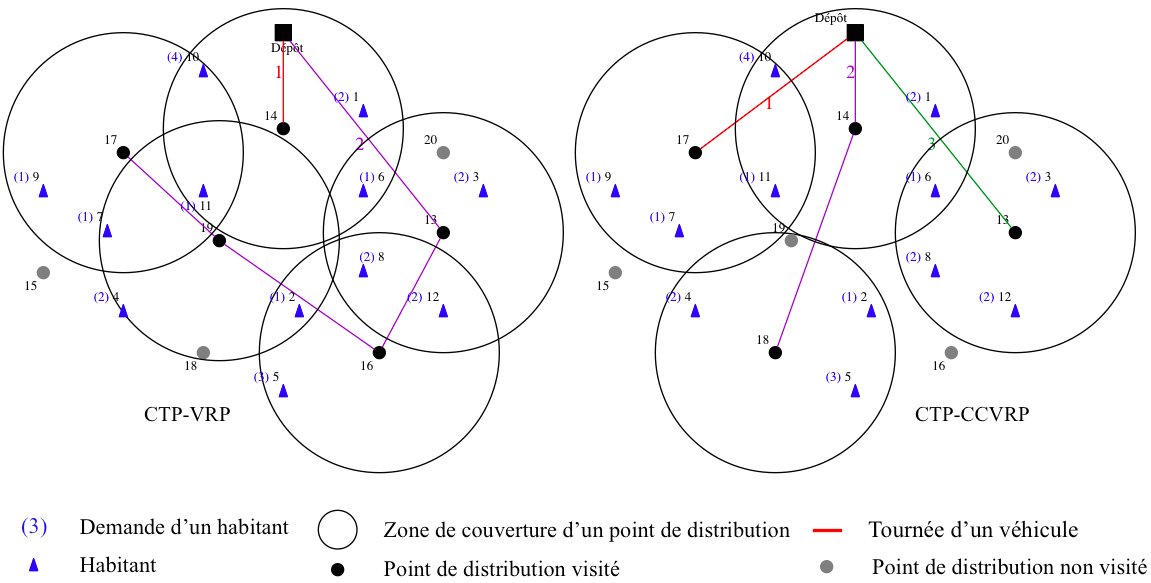
\includegraphics[width=0.6\textwidth]{figures/ctp-vrp_vs_ctp-ccvrp}
% \end{figure}
\item[2015, stage fin M1] (4 mois, Mobigis) Algorithme de plus court chemin pour le covoiturage
\item[2014, stage fin L3] (5 mois, IRAP) Création d'un autoguidage pour les coronographes du Pic du Midi 
\end{description}
\end{frame}





\begin{frame}{Mes motivations}

Pourquoi ce sujet ?
\begin{itemize}
\item Mêle \alert{tous les domaines} de ma formation (optimisation, graphes, algorithmie, traitement d'images, apprentissage automatique)
\item Collaboration \alert{mathématiques-informatique} enrichissante
\end{itemize}
Et pour la suite...
\begin{itemize}
\item Objectif professionnel : \alert{Chercheur} (Inria, CNRS) ou enseignant-chercheur ou R\&D (CNES, Thalès)
\end{itemize}
\end{frame}



\plain{Sujet de thèse}



\begin{frame}{Problématique}
\begin{itemize}
\item La \alert{représentation parcimonieuse} permet de débruiter, décrire, compresser, classifier
\item Un dictionnaire peut permettre de représenter l'image parcimonieusement
\item Deux catégories de dictionnaires. Exemples de méthodes :
\begin{table}[] \centering
\begin{tabular}{@{}lcc@{}}
\toprule
 & Rapide & Adaptatif \\ \midrule
Transformée en cosinus (analytique) & \Geq{\cmark} & \Req{\xmark}\\
K-SVD (appris) & \Req{\xmark} & \Geq{\cmark} \\ \bottomrule
\end{tabular}
\end{table}
\item Un dictionnaire \alert{adaptatif et rapide} ?
\end{itemize}
\end{frame}




\begin{frame}{État de l'art de l'équipe}
Dans \citetitle{chabiron_optimization_2016} (\alert{thèse CIMI} précédente), le dictionnaire $\D$ est défini par
\begin{columns}
\begin{column}{0.60\textwidth}
\\
$\D \code = \Req{\sum_{f \in \text{ Feuilles}}} \code^{\Req{f}} * \underbrace{h^{\Req{f}}* \dots* h^{r}}_{\textrm{de la racine à la feuille}}$
\end{column}
\begin{column}{0.50\textwidth} { \small
\Req{\xmark} $\D \code$ sans structure $\Rightarrow O(N^2)$\\
\Geq{\cmark} $\D \code$ avec structure d'arbre $\Rightarrow O(N)$
}
\end{column}
\end{columns}

	\begin{columns}
	\begin{column}{0.30\textwidth}
    	\begin{figure}\centering
	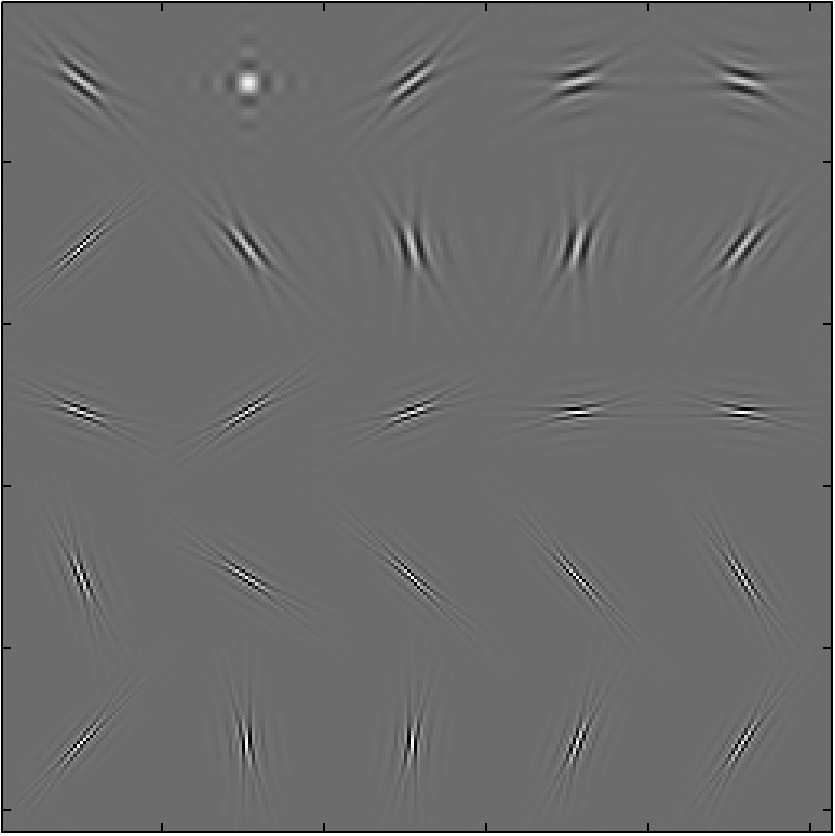
\includegraphics[width=1\linewidth]{figures/curv_datafit2.png}
	\caption{Image $\data$ sur laquelle on apprend le dictionnaire}
	\end{figure}

	\end{column}
	\begin{column}{0.30\textwidth}
		\begin{tikzpicture}[remember picture,overlay]
			\path[draw=black,thick,->]<3-> (0,0) -- (3,0);
		\end{tikzpicture}
		\begin{center}
			Optimisation de $\D$
            	\begin{equation*} {\small
\underset{\substack{(h^\text{e})_{e}}}\min
	\norm{\Req{\sum_{f \in \leaves}} \code^{\Req{f}} * h^{*\Req{f}} -\data}{2}^2
    }
	\end{equation*}
		\end{center}

	\end{column}
    
	\begin{column}{0.50\textwidth}
	\begin{figure}\centering
	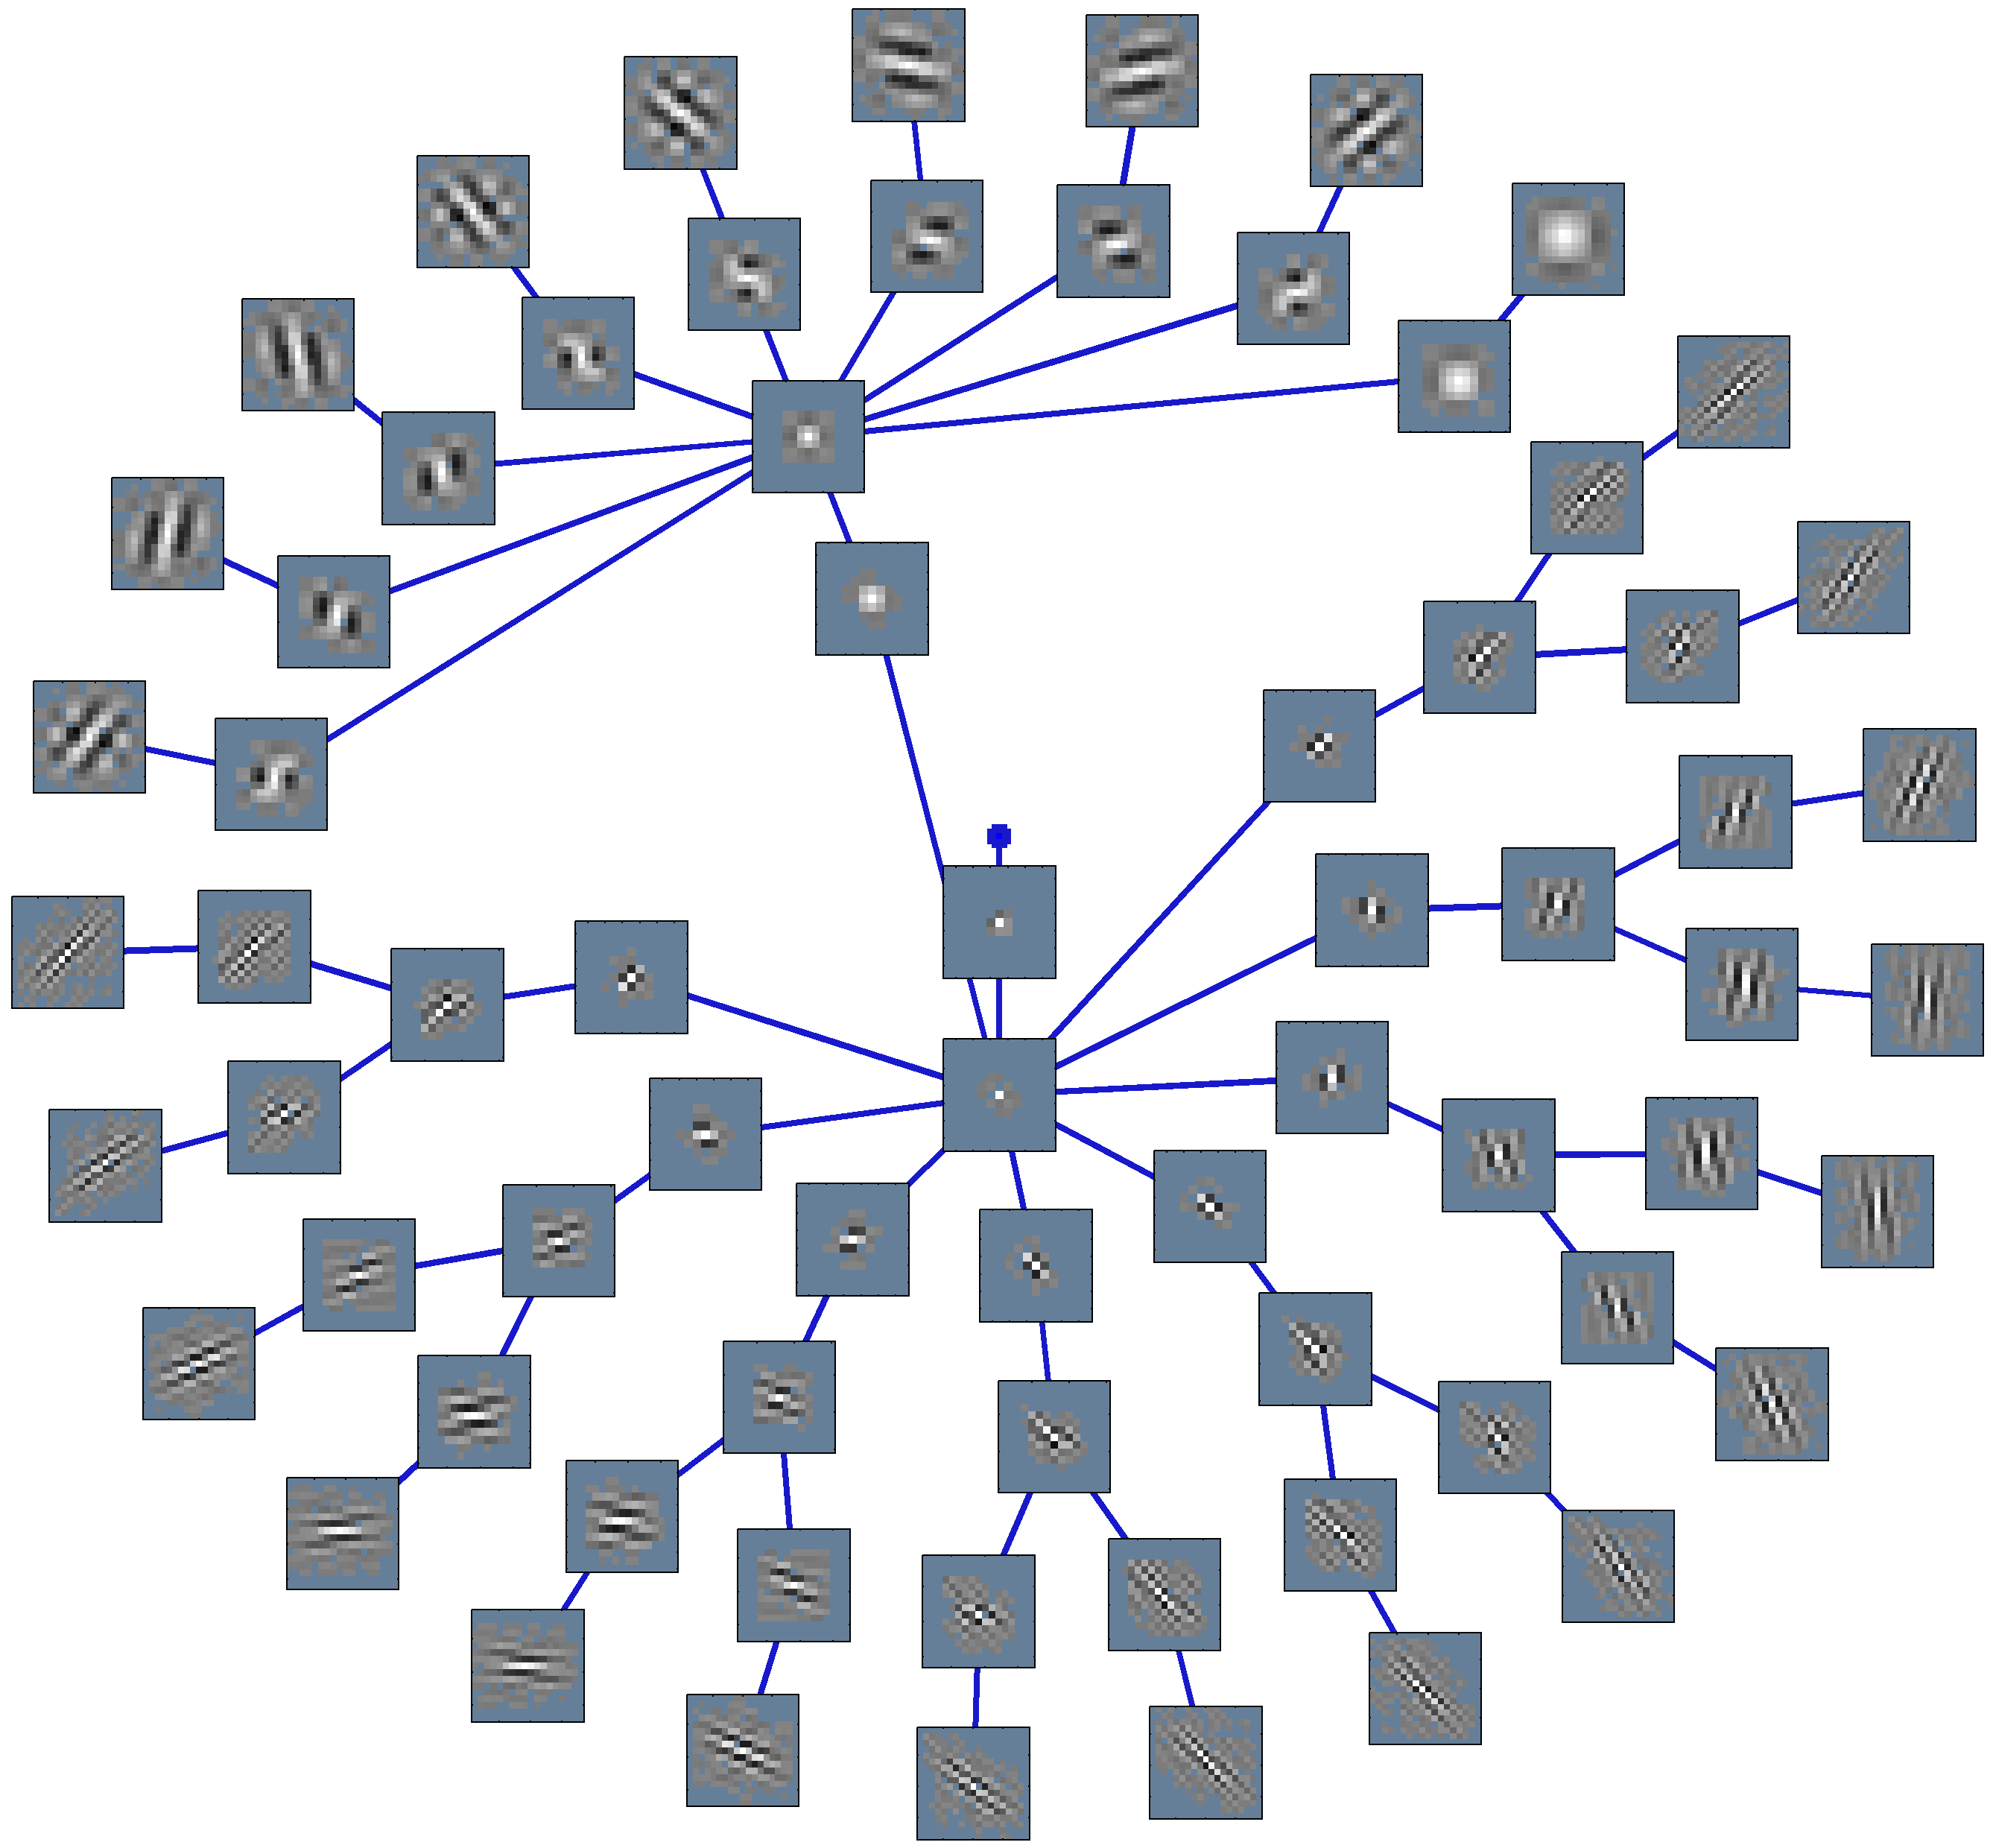
\includegraphics[width=1\linewidth]{figures/approx_MotherTree.png}
	\caption{Arbre représentant $\D$}
	\end{figure}
	\end{column}
	\end{columns}
    

    
\end{frame}

\begin{frame}{Les verrous à lever}
Verrous :
\begin{itemize}
\item l'arbre est créé \alert{à la main}
\item les supports\footnote{Support = endroit où le noyau de convolution peut être non-nul} sont aussi choisis \alert{à la main}
\end{itemize}
Conséquences :
\begin{itemize}
\item Méthode \alert{pas assez adaptative}
\item Difficile d'obtenir une bonne approximation de l'image pour certains $\data$
\end{itemize}

\end{frame}

\begin{frame}{Le travail à effectuer}
\begin{enumerate}
\item \alert{Optimiser} les supports des noyaux de convolution
\item \alert{Optimiser} l'arbre en créant/regroupant certains arcs
\item Passer d'un arbre à un \alert{graphe} pour des atomes plus complexes
\end{enumerate}
\end{frame}


\begin{frame}{En quelques mots...}
\begin{itemize}
\item un premier pas dans la recherche (TER M1)
\item projet d'\alert{enseigner} durant la thèse et objectif enseignant-chercheur
\item thèse CIMI mêlant $\underbrace{\text{\alert{informatique}}}_{\text{ma formation}}$ et $\underbrace{\text{\alert{mathématiques}}}_{\text{stage de M2}}$
\end{itemize}
\vfill
\hfill Merci de votre attention
\end{frame}

\appendix

\begin{frame}[allowframebreaks,noframenumbering]
\frametitle{Bibliographie de l'équipe}
\nocite{*}
\printbibliography[heading=none]
\end{frame}


\end{document}